\chapter{CI/CD in Banken}
\label{ch:chapter04}

\section{Nachvollziehbarkeit der SEU}
Die \ac{SEU} sollte aus mehreren Gründen möglichst nachvollziehbar gestaltet werden. Eine flexible Umgebung setzt auch Wartbarkeit und Anpassungsfähigkeit voraus. Dies ist durch die Verwendung von gängigen Standards möglich. Systeme sollten möglichst unabhängig von einzelnen Verantwortlichen verständlich und offen sein. Eine Individualisierung von Systemen sollte möglichst vermieden werden. Sie sollten auf einen gemeinsamen Nenner gebracht werden.

Dadurch kann eine schnelle Anpassung der Systeme an neue Technologien und Methoden erfolgen. Gleichzeitig können Systeme für neue Geschäftsmodelle in kurzer Zeit weiterentwickelt werden. Während einer Störung der Systeme oder in Krisensituationen kann auch schnell reagiert werden.

Dies hat auch einen positiven Effekt auf interne Kontrollverfahren. Die Umgebung ist nicht nur verständlicher für den Prüfer sondern auch sicherer durch die Verwendung von bereits geprüften Standards.

Nachvollziehbarkeit wird in Banken auch für die Rückverfolgung von Softwareartefakten vorausgesetzt. In der Praxis müssen Ergebnisse aus der Entwicklung rückverfolgbar sein bis auf den Quellcode, der Anforderung und dem Prozess aus der sie entstanden sind.

\section{DevOps mit Mircroservices}
Daraus folgt, dass einzelne umfangreiche Systeme für die \ac{SEU} keine Flexibilität bieten. Für automatisierte Prozesse und skalierbare, flexible Umgebungen können die Anwendungen aus der \ac{SEU} in noch kleinere Module aufgeteilt werden. Insbesondere ist es wichtig, dass einzelne Komponenten der Integrationsplattform trennbar sind und unabhängig voneinander laufen. Komponenten sollten \enquote{self-contained} aufgebaut werden. In folge dessen sind sie flexibler können auch unabhängig voneinander skaliert werden. Das würde Engpässe erheblich reduzieren. Die Eliminierung von Abhängigkeiten sorgt für eine bessere Nachvollziehbarkeit, da hierbei gängige Standards angewendet werden können.

\paragraph{Repository für Artefakte}
Eine Standardsoftware hierfür die Anwendung Artifactory. Diese speichert in einem Snapshot die Ergebnisartefakte aus dem Build-Job und die zum erstellen verwendeten Artefakte. Das Artifactory wird ebenfalls verwendet, um Tools und Libraries für den Build zu beziehen. Dazu wird Artifactory entweder als Proxy für den Zugriff auf ausgesuchte öffentliche Repositories verwendet oder die Ressourcen werden in der Artifactory Instanz hinterlegt.

\section{Skalierung von Jenkins mit Kubernetes}
\label{jenkins:skalierung}
Üblicherweise werden Anwendungen in Kubernetes mit Replikas skaliert. Das heißt in der Praxis, dass eine neue Instanz der Anwendung erzeugt wird und ein Load-Balancer die Anfragen unter den verschiedenen Instanzen verteilt. Das resultiert in der vorwiegend horizontalen Skalierung von Anwendungen. 

Jenkins besteht bei einer Konfiguration mit verteilten Builds aus mehreren Komponenten. Ein Jenkins Master, welche die Anfragen bearbeitet und Build-Jobs triggert und ausführende Agenten für die Verteilung von Builds. Die Komponenten sollten getrennt voneinander skaliert werden, da sie vorwiegend für die ausführenden Komponenten erforderlich ist. 

Hierfür gibt es in Kubernetes mehrere Abstraktionsebenen. Die größte Einheit, die die ganze Architektur zusammenfasst ist der Cluster. Dieser besteht aus mehreren Knoten, die jeweils mehrere Pods beinhalten. Die Knoten sind virtuelle Maschinen und enthalten die Hardware. Innerhalb dieser Knoten werden die Container ausgeführt. Diese sind noch einmal unter Pods zusammengefasst, die eine Arbeitseinheit oder Service darstellen. 
\medskip
\\
Ein sinnvoller Ansatz ist die ganze Anwendung innerhalb eines Knotens aufzubauen und sie durch Replikas der Knoten zu skalieren. Dabei sollte die Anwendung modularisiert werden und in unabhängig voneinander skalierbare Microservices aufgeteilt werden. Anwendungen können komplex sein und ein Engpass entsteht in wenigen Bereichen, sodass nicht die ganze Anwendung repliziert werden muss. In der Praxis werden die Funktionen der Anwendung in mehreren Containern aufgeteilt, die miteinander kommunizieren. Die Replikation von Containern bewirkt, dass Anwendungen nur in den Komponenten skaliert werden, in der es erforderlich ist. Diese Praxis schafft Redundanzen ab und und sorgt für einen Wirkungsgrad in der Nutzung von IT-Ressourcen.


%
\paragraph{Google Kubernetes Engine}

\begin{figure}[htbp]
 \centering
 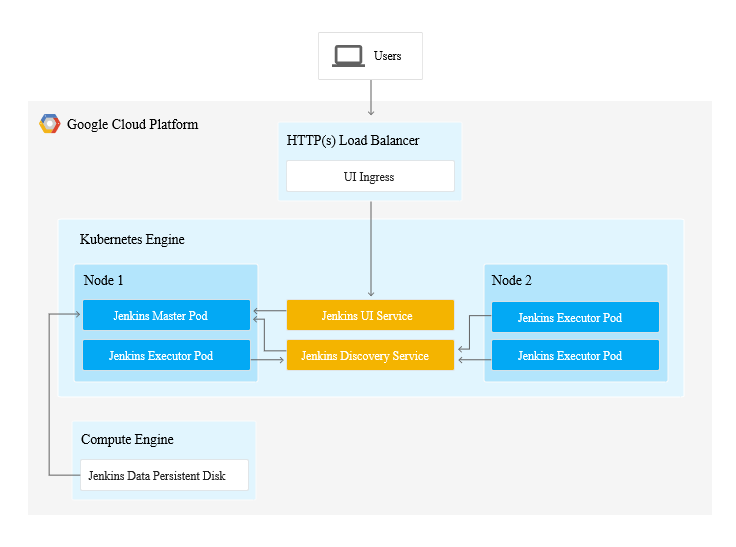
\includegraphics[width=1.0\textwidth]{gfx/jenkins-kubernetes-architecture.png}
 \caption{Deployment von Jenkins in einem Kubernetes Cluster mit mehreren Knoten \cite{Google:GKEJenkins}\label{fig:gkejenkins}}
\end{figure}

Google beschreibt in \cite{Google:GKEJenkins} einen Ansatz für eine skalierbare Architektur von Jenkins mit der \ac{GKE}.

In Abb. \ref{fig:gkejenkins} werden die Komponenten in mehreren Knoten, genannt Nodes zusammengefasst. In Node 1 befindet sich der Jenkins Master. Innerhalb dieses Nodes kann der Jenkins Master repliziert werden. Im gleichen Node oder in weiteren Nodes können die Jenkins Agenten, genannt Jenkins Executor, erzeugt werden.

Der Load Balancer aus der \ac{GKE} arbeitet vollautomatisch und erfordert nur wenige Parameter zur Konfiguration. Das reduziert den Aufwand in der Entwicklung dieser Architektur erheblich.

So lange in einem Node genug Ressourcen frei sind können weitere Container in so genannten Pods erzeugt werden. Zudem können beliebig viele weitere Nodes aktiviert oder erzeugt werden. Ein Node ist in \ac{GKE} eine virtuelle Maschine aus der Computing Engine.
\medskip
\\
Daraus resultiert eine hohe Flexibilität für die Skalierung der Anwendungen. Diese können sowohl vertikal anhand der Ressourcen von den Nodes, als auch Horizontal über die Aktivierung von weiteren Nodes oder Pods skaliert werden. Vor allem bestehen für die horizontale Skalierung mehrere Abstraktionsebenen.

\paragraph{Minikube}

\subsection{Anlegen eines Kubernetes Clusters für Jenkins}
Pathania beschreibt in \cite{Pathania2017}, wie Jenkins mit \ac{GCP} und Kubernetes und Docker skaliert werden kann. Hierbei geht er genau auf die Konfiguration von Kubernetes und der \ac{GCP} ein.



\paragraph{Jenkins Master-Agent Konfiguration}


\paragraph{Sonstige Konfigurationen}

\subsection{Jenkins Agents}

\paragraph{Virtuelle Maschinen}

\paragraph{Docker}

\paragraph{Minimale Images}

\subsection{Layering}
